\subsection{Problems}

\vspace{1cm}
\noindent {\bf Problem \thesection.\theprob}\stepcounter{prob}

A pump delivers water from a low-pressure steam boiler as shown in the figure below. Calculate the required geodetic height of the reservoir to avoid cavitation! The pipeline losses are to be taken into account.

\begin{tabular}{cc}
    \begin{minipage}{6cm}
	\begin{center}
	    \resizebox{5cm}{!}{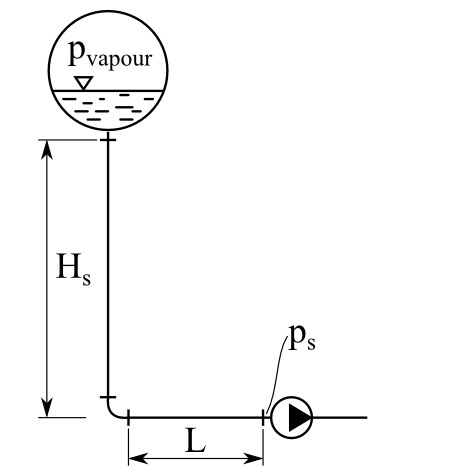
\includegraphics{Problem_solving/figs/PS_NPSH_figure2.png}}\\
	\end{center}
    \end{minipage}
& 

\begin{minipage}{9cm}
\begin{itemize}
\item mass flow rate: $\dot m=27 [kg/s]$, density of the hot water: $\rho=983 [kg/m^3]$
\item pipe: $L=10[m]$, $d=100[mm]$, $\lambda=0.02$ and the sum of loss factors is $\zeta=5$
\item pump: $H[m]=82-4800\,Q^2$, $\mathit{NPSH}[m]=1.6+1360\, Q^2$
\end{itemize}

\emph{Solution:} 

It's easy to calculate that\\
$Q=\dot m/ \rho=0.02747 [m^3/s]$ \\ 
$c_s=Q/A=3.5[m/s]$\\
$H=82-4800 \times 0.02747^2=78.38[m]$\\ 
$\mathit{NPSH}=1.6+1360 \times 0.02747^2=2.626[m]$ 

\end{minipage}
\end{tabular}

\vspace{0.5cm}

Bernoulli's equation between a surface point in the tank and the suction side of the pump reads:

\begin{equation*}
\frac{p_t}{\rho g} + \frac{0^2}{\rho g}+H_s\,=\,\frac{p_s}{\rho g} + \frac{c_s^2}{\rho g}+0+h'_{pipeline}
\end{equation*}

From the suction side of the pump to the impeller we have:

\begin{equation*}
\frac{p_s}{\rho g} + \frac{c_s^2}{2 g}\,=\,\frac{p_{vapour}}{\rho g} + e_s + \mathit{NPSH}
\end{equation*}

(Note that $e_s=0$ as the configuration is horizontal.) Putting the above two equations together, we have

\begin{equation*}
\mathbf{H_s} =-\frac{p_t-p_{vapour}}{\rho g} + h'_{pipe} + \mathit{NPSH}, \quad \text{where} \quad h'_{pipe} = \frac{c_s^2}{2g}\left( \lambda \frac{\mathbf{H_s}+L}{d}+\zeta \right),
\end{equation*}

thus,

\begin{equation*}
H_s =\left( 1-\frac{c_s^2}{2g} \frac{\lambda}{d} \right)^{-1} \left[ \mathit{NPSH} + \frac{c_s^2}{2g} \left( \frac{\lambda L}{d}+\zeta \right) \right]=\dots=8.116[m]
\end{equation*}

Thoma's cavitation coefficient is $\sigma=\mathit{NPSH}/H=0.03355[-]$.

\vspace{1cm}
\noindent {\bf Problem \thesection.\theprob}\stepcounter{prob}

Calculate the required pipe diameter to avoid cavitation, if the pump delivers $Q=30\,\mathrm{dm^3/s}$ water from a closed tank, where the pressure (above the water level) is $p=40\,\mathrm{kPa}$. The equivalent pipe length on the suction side is $5m$, the friction coefficient is $\lambda=0.02$, the suction flange of the pump is $3\,\mathrm{m}$ below the water level. The vapour pressure at the water temperature is $2.8\,\mathrm{kPa}$. The required net positive suction head is $\mathit{NPSH}_r=3.2\,\mathrm{m}$. (The standard pipe diameter series is: DN 40, 50, 65, 80, 90)

\noindent Solution:

\noindent The sketch of the installation is shown in Figure~\ref{fig:NPSH_figure1}

\begin{figure}[ht]
\centering
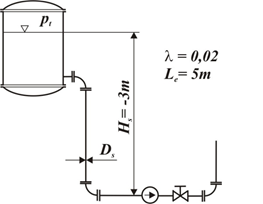
\includegraphics[width=0.37\textwidth]{Problem_solving/figs/PS_NPSH_figure1.png}
\caption{\label{fig:NPSH_figure1}Installation of the apparatus.}
\end{figure}

\begin{itemize}
\item $\mathit{NPSH}_a=\frac{p_t-p_v}{\rho g}-H_s-h'_s\quad\rightarrow h'_s=\frac{p_t-p_v}{\rho g}-H_s-\mathit{NPSH}_r$
\item $h'_s=\lambda \frac{L_e}{D_s}\frac{c^2_s}{2g}=\lambda \frac{L_e}{D_s}\frac{8Q^2}{D^4_s g \pi^2}$
\item $D_s=0.073m\rightarrow D_s=80\,\mathrm{mm}$
\end{itemize}

\vspace{1cm}
\noindent {\bf Problem \thesection.\theprob}\stepcounter{prob}

Find the required suction side height of the pump that conveys water from an open surface reservoir at $Q=180m^3/h$ flow rate the head is $H=30m$ the required net positive suction head $\mathit{NPSH}_r=5.03m$. The temperature of the water is $T=23^\circ$ the ambient pressure is $p_0=1023mbar$. The hydraulic loss of the suction side pipe can be calculated from $h'_s=652[s^2/m^5]Q^2$ while the vapour pressure $p_v (\mathrm{kPA})=1.704+0.107(t-15)+0.004(t-15)^2$. Find the Thoma cavitation number. (Solution: $H_s=3.481m$, $\sigma=0.1677$)

